% Using a4paper and 12pt font by default
\documentclass[12pt, a4paper]{article}

%Includes "References" in the table of contents
\usepackage[nottoc]{tocbibind}

% Use more than one optional parameter in a new commands
\usepackage{xargs}

% Coloured text etc.
\usepackage[pdftex,dvipsnames]{xcolor}

% Pictures and /includegraphics
\usepackage{graphicx}
% Links in the table of contents + other stuff
\usepackage[hidelinks, linktoc=all]{hyperref}

% Support multi-page code listings
\usepackage[all]{hypcap}
\usepackage{subcaption}

% Times New Roman font
\usepackage[T1]{fontenc}
\usepackage{newtxmath,newtxtext}

% Margins
\usepackage[margin=2.5cm]{geometry}

% Interline
\usepackage{setspace}
\setstretch{1.5}

% Footnotes
\usepackage[bottom]{footmisc}

% Captions
\usepackage{caption}

% Todo notes
\usepackage[colorinlistoftodos,prependcaption,textsize=tiny]{todonotes}
\newcommandx{\unsure}[2][1=]{\todo[linecolor=red,backgroundcolor=red!25,bordercolor=red,#1]{#2}}
\newcommandx{\change}[2][1=]{\todo[linecolor=blue,backgroundcolor=blue!25,bordercolor=blue,#1]{#2}}
\newcommandx{\info}[2][1=]{\todo[linecolor=OliveGreen,backgroundcolor=OliveGreen!25,bordercolor=OliveGreen,#1]{#2}}
\newcommandx{\improvement}[2][1=]{\todo[linecolor=Plum,backgroundcolor=Plum!25,bordercolor=Plum,#1]{#2}}

% Code highlighting
\usepackage{minted}
\usemintedstyle{tango}
\newcommandx{\listcode}[2][1=]{\bgroup\inputminted[linenos, breaklines=true, fontsize=\scriptsize]{python}{#1}\captionof{listing}{#2}\egroup}
\newcommandx{\listcodecont}[2][1=]{\bgroup\inputminted[linenos, breaklines=true, fontsize=\scriptsize,firstnumber=last]{python}{#1}\captionof{listing}{#2}\egroup}

% New line after paragraph title
\newcommandx{\myparagraph}[1]{\paragraph{#1}\mbox{}}

% List stuff easily
\usepackage{multicol}
\usepackage[sharp]{easylist}

\let\OldEasylist\easylist
\let\OldEndEasylist\endeasylist
\renewenvironment{easylist}{%
    \OldEasylist%
    \ListProperties(Progressive*=3ex, Start1=1)%
}{%
    \OldEndEasylist%
}%


\begin{document}

% Title page

\begin{titlepage}
\end{titlepage}

\newpage

% Table of Contents

\tableofcontents

\newpage
% Misc
\newpage
\listoftodos[Temporary Notes]

% Abstract

\begin{abstract}

\end{abstract}



%===============================================================================
\newpage
\section{INTRODUCTION}
%===============================================================================

%-------------------------------------------------------------------------------
\subsection{State of the Art in Data Science}
%-------------------------------------------------------------------------------
\improvement[inline]{Use stuff from the presentation}
\begin{easylist}
# Why is data analysis useful?
## Modern amounts of data explanation
## Data analysis explanation
# What tools are used to deal with large amounts of data?
## Traditional - ETL and DW (microsoft, qlikview, ...)
## Explorational - spark, R, python, matlab
# Why choose python?
## Advantages and disadvantages of using python
## Overview of chosen packages
\end{easylist}

\change[inline]{Rewrite everything}
%-------------------------------------------------------------------------------
\subsection{Goals of the Research}
%-------------------------------------------------------------------------------
 In the modern world, big data and machine learning are becoming more and more prominent as companies such as Facebook, Google and Amazon gather and analyze all sorts of data from their users. But which tools are they using to do it?

Right now, the two main languages in data science are \texttt{Python} and \texttt{R}, while \texttt{Matlab} is also quite popular despite only being used in the academic environment.

This work's objective is to show how to use the Python 3 programming language in dealing with different kinds of data, and to help clarify any problems that might come up. It may be useful for long-term users of other languages that want to try Python out as well as users of Python 2, support for which will be stopped in 2020.
%-------------------------------------------------------------------------------
\subsection{Thesis Overview}
%-------------------------------------------------------------------------------
This work will be split into three parts, each working with a different dataset.

In the first part, I'll show you how to obtain, plot and predict stocks based on the last 17 years' worth of stock data from NYSE\footnotemark. I'll also cover some common problems that might occur when one is trying to deal with such amount of data.
\footnotetext{New York Stock Exchange}

In the second part, I'll cover scraping facebook's API, and plotting geolocation data of their events. I'll also discuss some problems that might occur while trying to download data, as well as how to use latest tools from Python (like the asyncio library) to speed up the data gathering part greatly. I'll also give you a brief overview of the current data visualization landscape, and show you which plotting packages are the best to use when dealing with geolocation data.

In the third part, I'll delve into the YouTube system, and will try to download and analyze their videos.

Lastly, the fourth part will contain conclusions.

%===============================================================================
\newpage
\section{TABULAR DATA ANALYSIS}
%===============================================================================
%-------------------------------------------------------------------------------
\subsection{Project Overview}
%-------------------------------------------------------------------------------
\begin{easylist}
# Goals
## Describe the project
# Obtaining the data (pandas-datareader)
# Traditional stock visualizations (matplotlib)
# Stock correlation matrix (matplotlib)
# LSTM training (keras)
\end{easylist}

%-------------------------------------------------------------------------------
\newpage
\subsection{Data gathering (pandas-datareader)}
%-------------------------------------------------------------------------------

%-------------------------------------------------------------------------------
\newpage
\subsection{Traditional stock visualizations (matplotlib)}
%-------------------------------------------------------------------------------

%-------------------------------------------------------------------------------
\newpage
\subsection{Stock correlation matrix visualization (matplotlib)}
%-------------------------------------------------------------------------------

%-------------------------------------------------------------------------------
\newpage
\subsection{Predictive analysis with a LSTM neural network (keras)}
%-------------------------------------------------------------------------------



%===============================================================================
\newpage
\section{GRAPH DATA ANALYSIS}
%===============================================================================
%-------------------------------------------------------------------------------
\subsection{Project Overview}
%-------------------------------------------------------------------------------
\begin{easylist}
# Goals
## to show how to run community detection algorithms in igraph
## to show how to plot the communities using two different methods - datashader  (larger data) and cairo (smaller data)
## to show how to make the communities visually separatable and how to incorporate node weights in the plot
# Tools(Libraries) used
## Why I chose igraph
\end{easylist}

\myparagraph{Packages needed}
\begin{easylist}
  # igraph
  # cairocffi
\end{easylist}

%-------------------------------------------------------------------------------
\newpage
\subsection{Preprocessing and igraph creation}
%-------------------------------------------------------------------------------
\begin{easylist}
# Importing the data form konekt
# Optimizing edges renaming with numpy vectorize/jit
\end{easylist}

%-------------------------------------------------------------------------------
\newpage
\subsection{Community detection (igraph)}
%-------------------------------------------------------------------------------

%-------------------------------------------------------------------------------
\newpage
\subsection{Plotting large graphs (datashader)}
%-------------------------------------------------------------------------------
%- - - - - - - - - - - - - - - - - - - - - - - - - - - - - - - - - - - - - - - -
\subsubsection{Simple plot}
%- - - - - - - - - - - - - - - - - - - - - - - - - - - - - - - - - - - - - - - -
\improvement[inline]{Add a note about how datashader failed to plot the entire graph and why it's not a good idea in the first place (hard to see the points)}

%- - - - - - - - - - - - - - - - - - - - - - - - - - - - - - - - - - - - - - - -
\subsubsection{Plotting communities}
%- - - - - - - - - - - - - - - - - - - - - - - - - - - - - - - - - - - - - - - -



%-------------------------------------------------------------------------------
\newpage
\subsection{Plotting small graphs (igraph)}
%-------------------------------------------------------------------------------
%- - - - - - - - - - - - - - - - - - - - - - - - - - - - - - - - - - - - - - - -
\subsubsection{Goals and section overview}
%- - - - - - - - - - - - - - - - - - - - - - - - - - - - - - - - - - - - - - - -
\myparagraph{Goals}

\begin{enumerate}
  \item Show how to create a regular graph plot, and consider the idea that its simplicity may make it harder to read
  \item Show how to create a graph plot with marked communities on it, and compare it to the regular plot in terms of ease of read
  \item Show how to create a graph plot with marked communities that also shows the weight of its nodes, and compare this plot to the other two
\end{enumerate}

\myparagraph{Description}

In this section, I will show you how to plot a smaller (around 2000 nodes) portion of our graph using tools that are supported by igraph, in particular using its bindings to a C library called \improvement{citation needed} cairo. Since it is originally written in C and only provides an API that other languages can use, we will also have to use a package that will be able to connect python code to the C library itself. In this example, I'm using cairocffi as such package, hence the inclusion of \mintinline{python}{import cairocffi as cairo} in the starting import list. We have to import it as cairo, because otherwise igraph will attempt to use a different binding package, \mintinline{python}{pycairo}, which is quite outdated and can outright refuse to save vector images.

%- - - - - - - - - - - - - - - - - - - - - - - - - - - - - - - - - - - - - - - -
\subsubsection{Regular plot}
%- - - - - - - - - - - - - - - - - - - - - - - - - - - - - - - - - - - - - - - -
\myparagraph{Selecting vertices}

First thing that we have to do in this section is to select a subgraph for plotting. I have decided to settle on the subgraph of vertices with high degrees, because that meant that every node would be connected to many other nodes, and that can be a good example of how to deal with clutter on the plot.

In order to select this subgraph, you can use the \mintinline{python}{graph.vs.select(*args, **kwargs)} method in your graph. This method works differently based on what you pass it:\newline

\begin{enumerate}
  \item If you pass a list of integers into it \mintinline{python}{select([1,2,3])}, or skip the list and call \mintinline{python}{select(1,2,3)}, it will return vertices at those indexes
  \item If you pass a special keyword argument to it, it will select all nodes with a property that match that argument
  \item If you pass a function to it, it will call that function on every vertex and return all vertices that the function has returned \mintinline{python}{True} for
  \item If you don't pass anything into the function, it returns an empty list
\end{enumerate}

The select method has 8 special keyword arguments:
\begin{multicols}{2}
  \begin{itemize}
  \item \texttt{eq} - equal to
  \item \texttt{ne} - not equal to
  \item \texttt{lt} - less than
  \item \texttt{gt} - greater than
  \item \texttt{le} - less than or equal to
  \item \texttt{ge} - greater than or equal to
  \item \texttt{in} - value is in the given list
  \item \texttt{notin} - value is not in the given list
  \end{itemize}
\end{multicols}

Please note, that you have to include name of your property before the special keyword: \mintinline{python}{graph.vs.select(age_in=[19,20,21])}. You can see how I have used \mintinline{python}{gt} in the following example. The \mintinline{python}{_degree} you see in front of it is a semi-private variable (since no variable is truly private in python) that keeps track of the degree of the vertex.

\listcode[src/youtube/hdg/1_selecting.py]{Selecting nodes for the subgraph}

\myparagraph{Styling the resulting plot}

There are many different options to choose from if you want to change how the graph appears on the screen. They are originally available as keyword arguments that you can pass to the \mintinline{python}{ig.plot()} function, but I advocate for putting all of those kwargs in a separate dictionary, \improvement{move save\_fname to the dictionary too} since it takes away from the dissaray of having to include many options into one function call.

In this paper I will mainly focus on the layout option, as well as gloss over a couple of settings connected to the size of the vertices and edges, but if after reading this you will want to learn more about them, you can call \mintinline{python}{help(ig.plot)} while in a python interpreter to see the function's docstring.

One of the most important arguments provided to us is the layout one, since it changes how nodes and edges are positioned in the resulting plot. It is possible to choose from the following layouts\footnote{Visual comparison is available at the page} \improvement{add visual comparison}:

\begin{multicols}{2}
  \begin{itemize}
  \item Circle layout
  \item Star layout
  \item Grid layout
  \item Fruchterman Reingold layout
  \item Fruchterman Reingold grid layout
  \item DrL layout
  \item Graphopt layout
  \item Kamada Kawai layout
  \item Large Graph layout
  \item Sugiyama layout
  \item Random layout
  \item Reingold Tilford layout (for trees)
  \item Bipartite layour (for 2-layer graphs)
  \end{itemize}
\end{multicols}

As you can see in the listing, other options are responsible for things like edge width, vertex size and shape, where to save the file, et cetera. The \texttt{bbox} argument is responsible for how big your final plot is going to be (in another words, it is declaring a limiting box on a figure that no vertex can cross). The \texttt{target} keyword argument is also very useful - it specifies the name of the file that your final chart will be stored in, and supports multiple file extentions (PDF, SVG, PNG).  In the next section I will also explain you how to add a color palette to the dictionary in order to distinguish the communities that we will detect.

\listcodecont[src/youtube/hdg/2_style_dict.py]{Creating a style dictionary}

\myparagraph{Plotting and saving the resulting plot to a file}

Since we have already constructed the keyword argument dictionary for the plot function, the rest becomes very clean and easy - just pass it to the function while remembering to unroll it to convert it to key-value pairs.

\listcodecont[src/youtube/hdg/3_plotting.py]{Plotting the image}

\begin{figure}[hb]
    \centering
    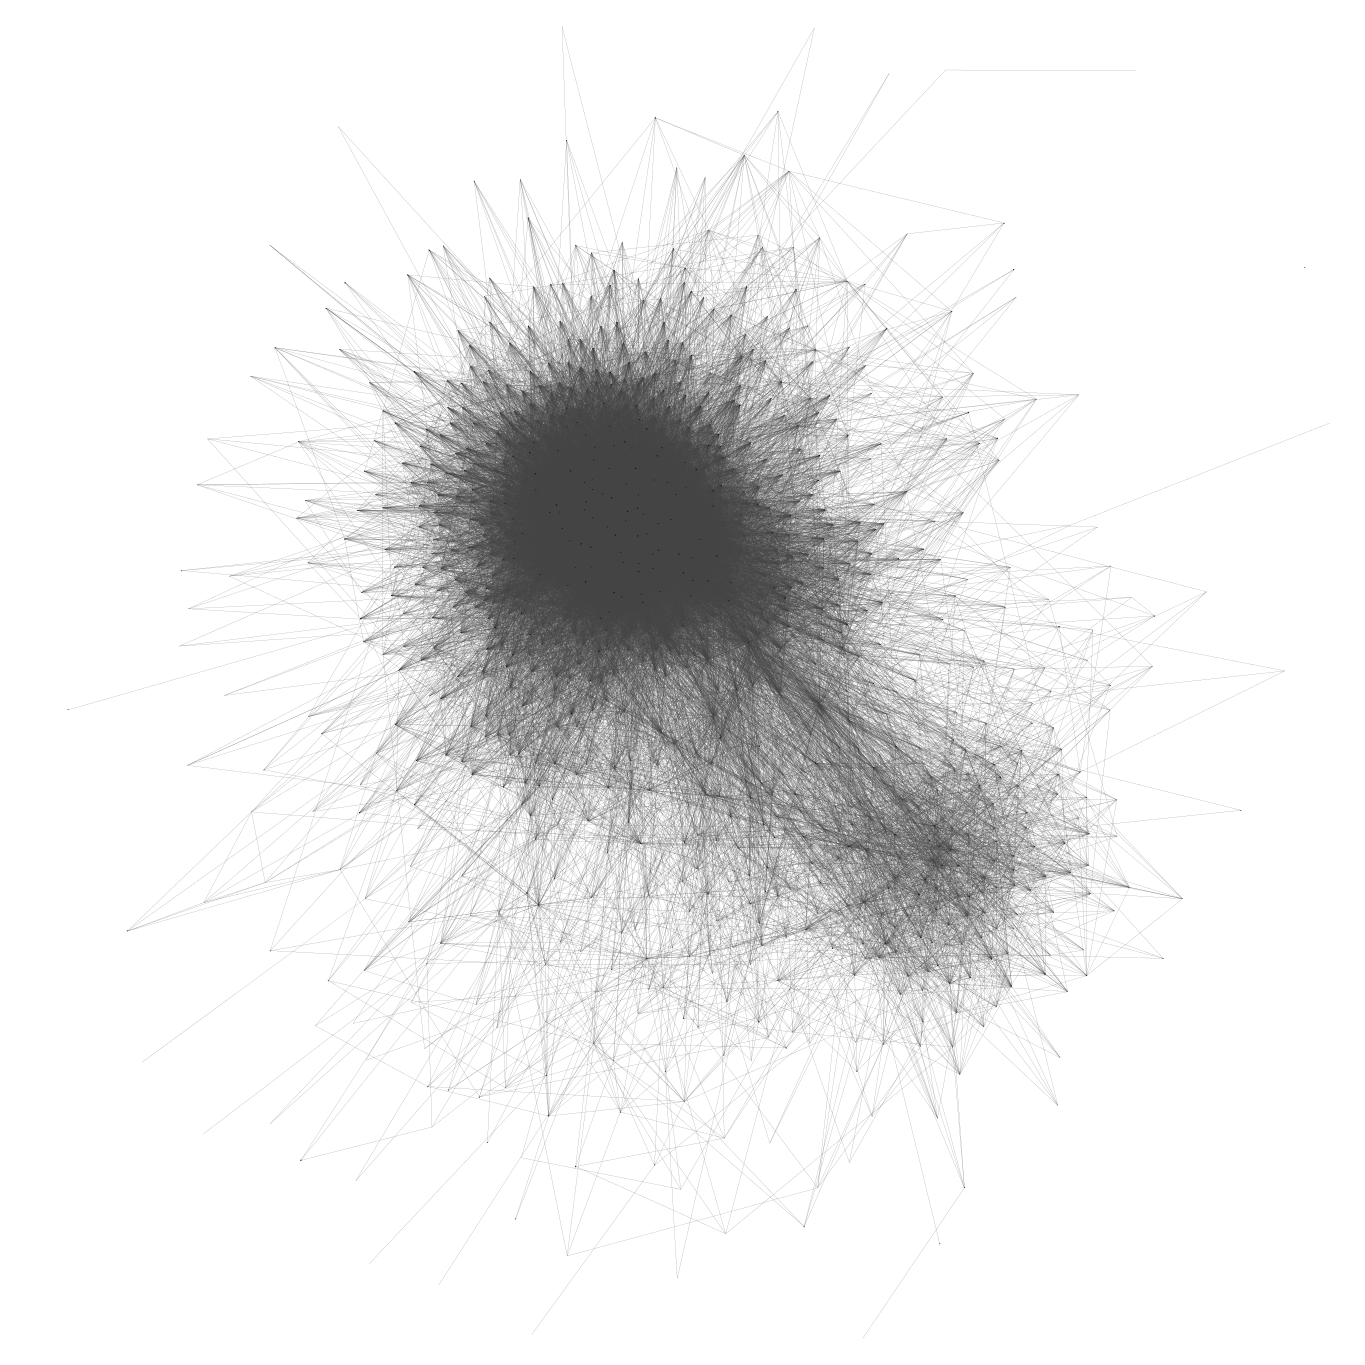
\includegraphics[width=\textwidth]{src/youtube/hdg/hdg_simple}
    \caption{Regular plot (Fruchterman Reingold layout)}
    \label{fig:hdg_simple}
\end{figure}

\myparagraph{Reviewing the results}

While igraph makes it quite easy to plot regular plots like these, they don't provide one with much insight into the data itself. While you could look at the picture made using the Fruchterman-Reingold layout, and detect two major communities in the network with a naked eye, other layouts aren't as simple to read. Furthermore, most of them look just black balls and are quite chaotic, which is a pretty common problem when dealing with plotting graphs.



\begin{multicols}{2}
  {\centering
  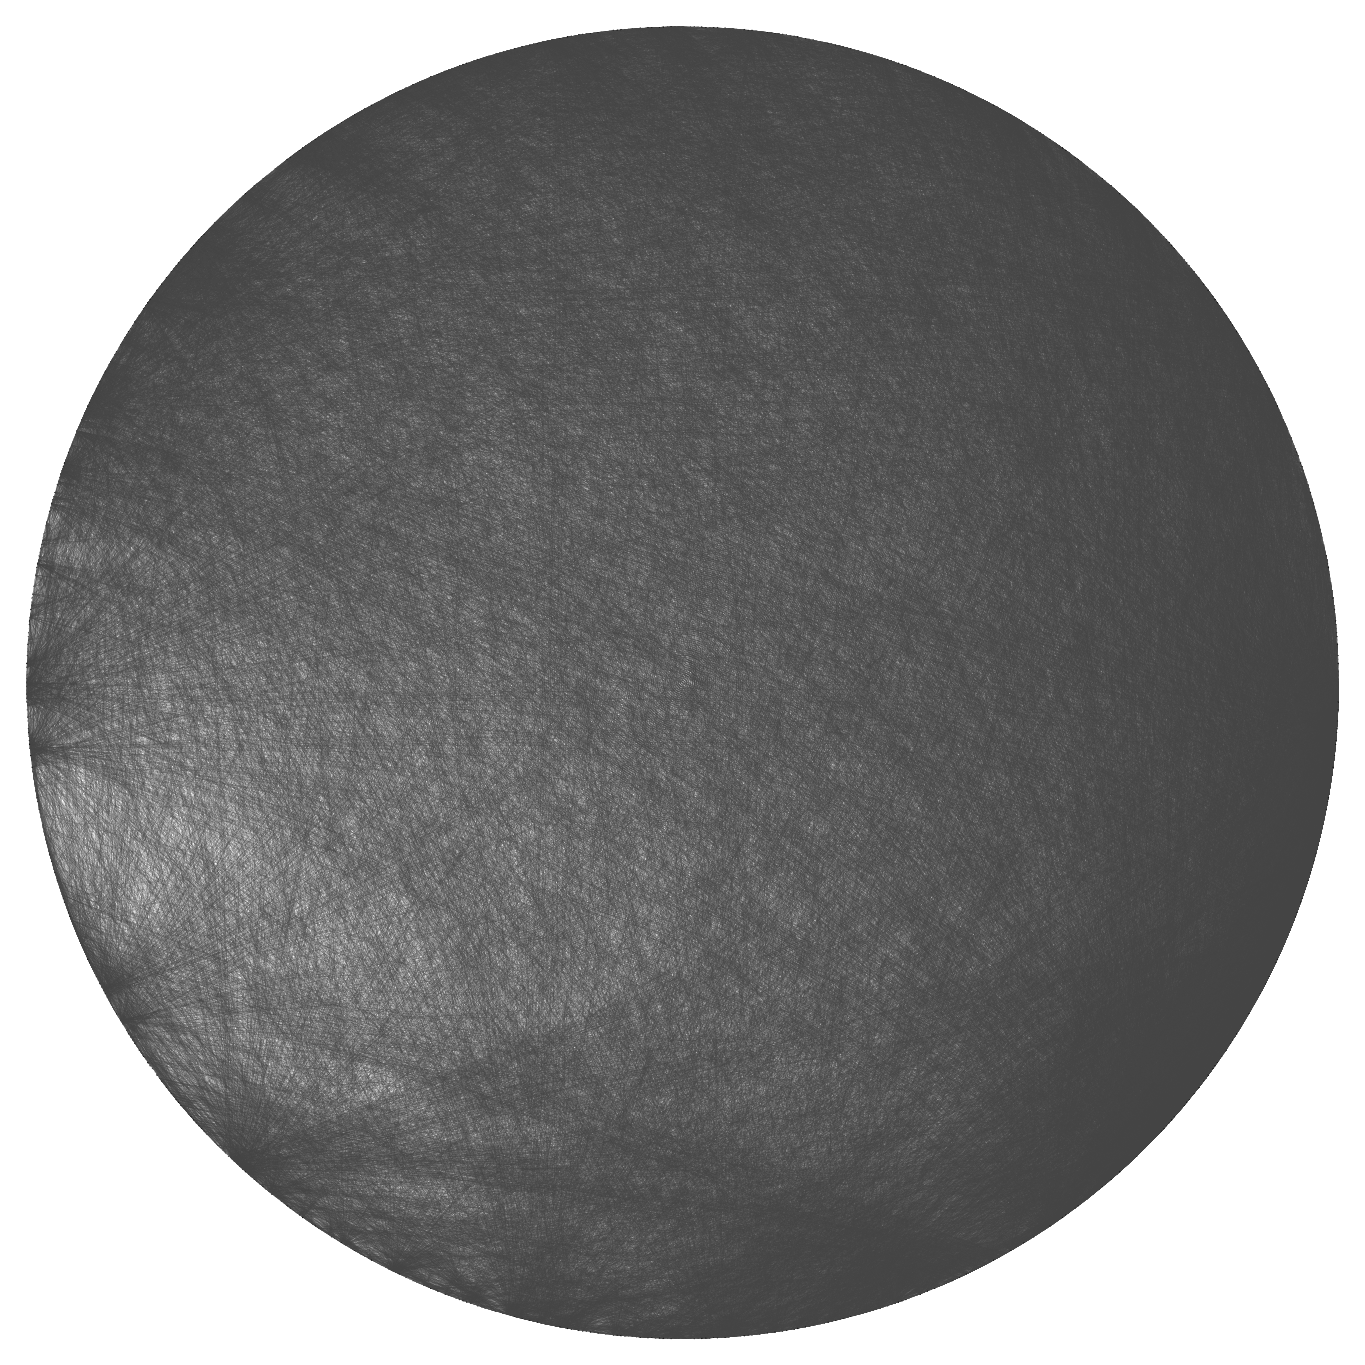
\includegraphics[width=\columnwidth]{src/youtube/hdg/comp/1_plot_crc}\\
  \captionof{figure}{Circular layout}
  \label{fig:hdg_c1}}
  {\centering
  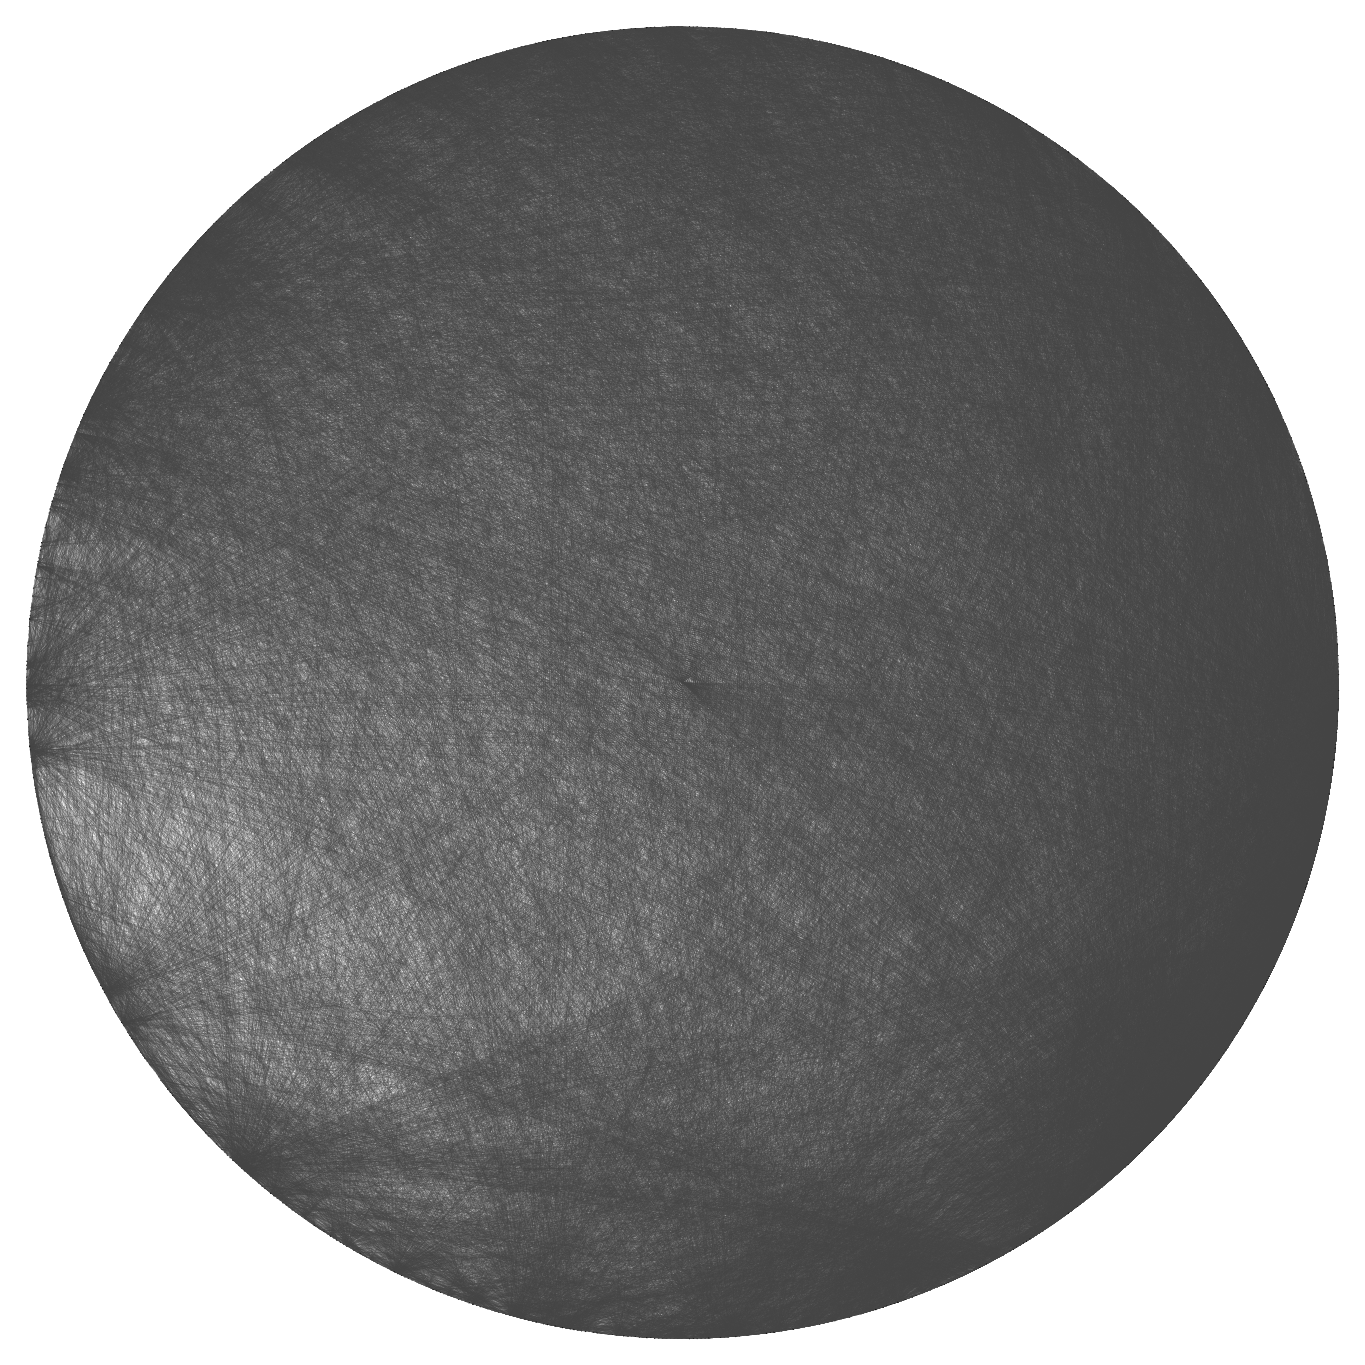
\includegraphics[width=\columnwidth]{src/youtube/hdg/comp/2_plot_str}\\
  \captionof{figure}{Star layout}
  \label{fig:hdg_c2}}
\end{multicols}
\begin{multicols}{2}
  {\centering
  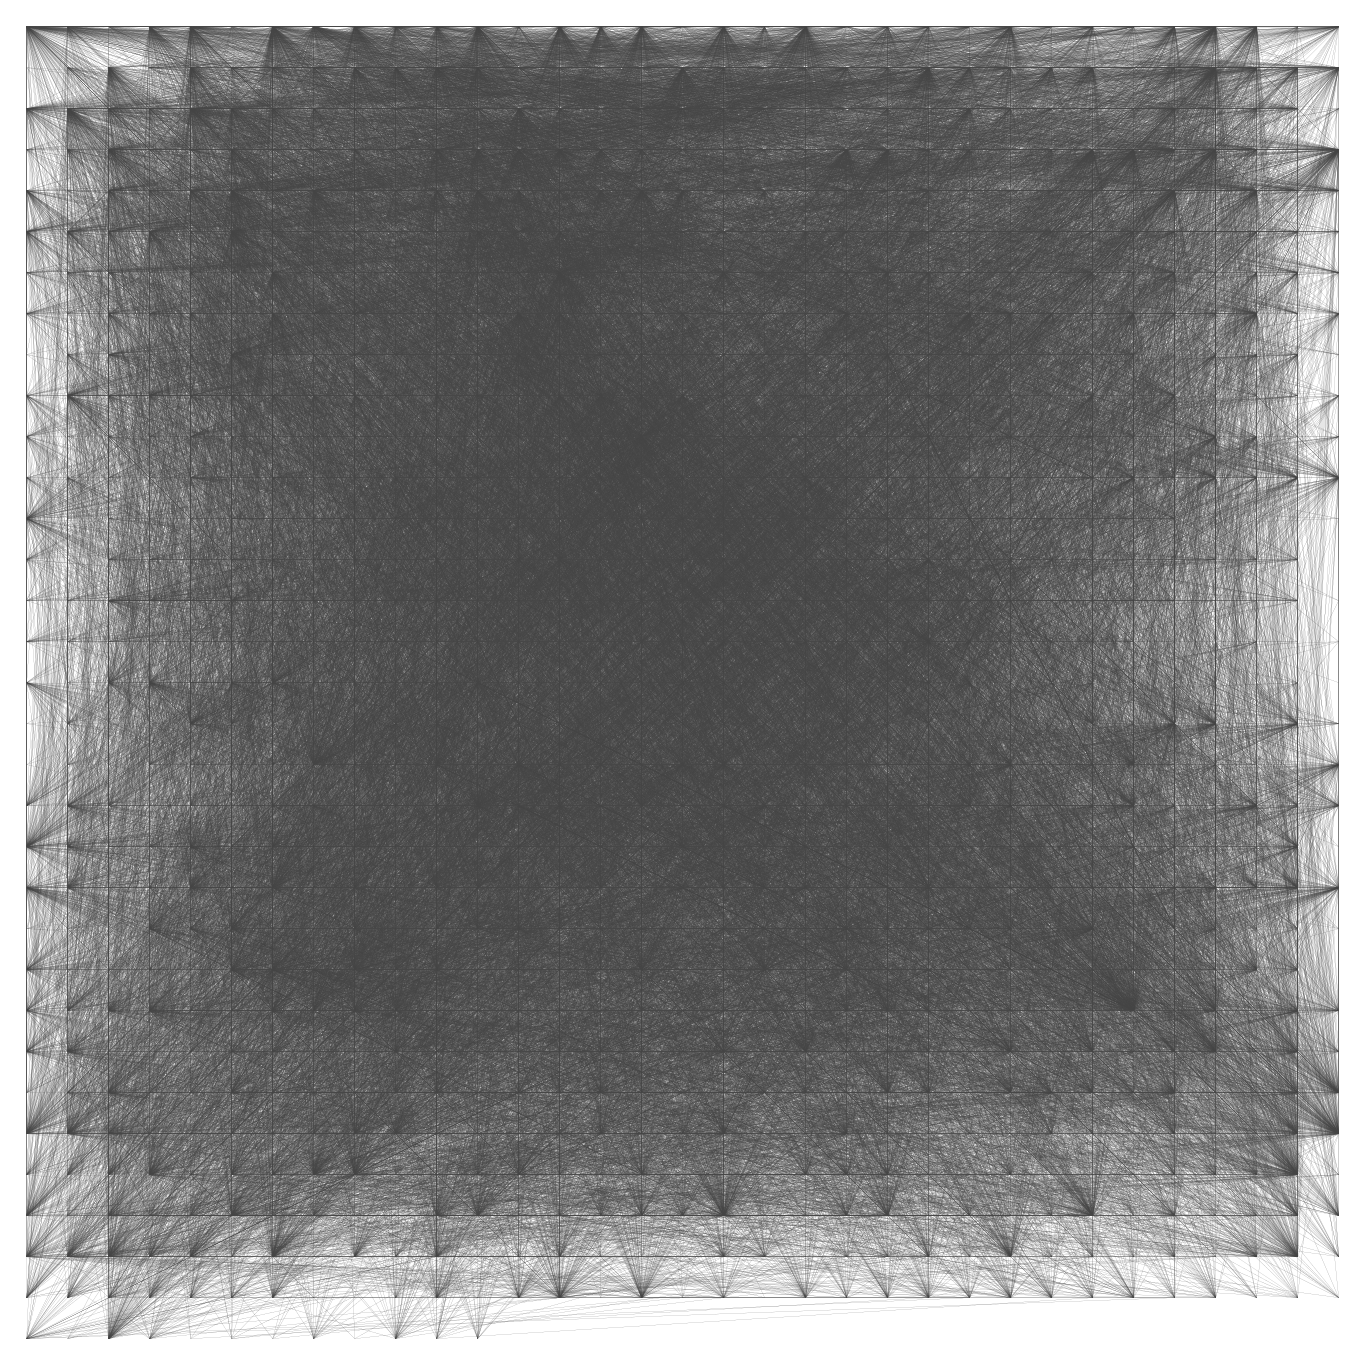
\includegraphics[width=\columnwidth]{src/youtube/hdg/comp/3_plot_grd}\\
  \captionof{figure}{Grid layout}
  \label{fig:hdg_c3}}
  {\centering
  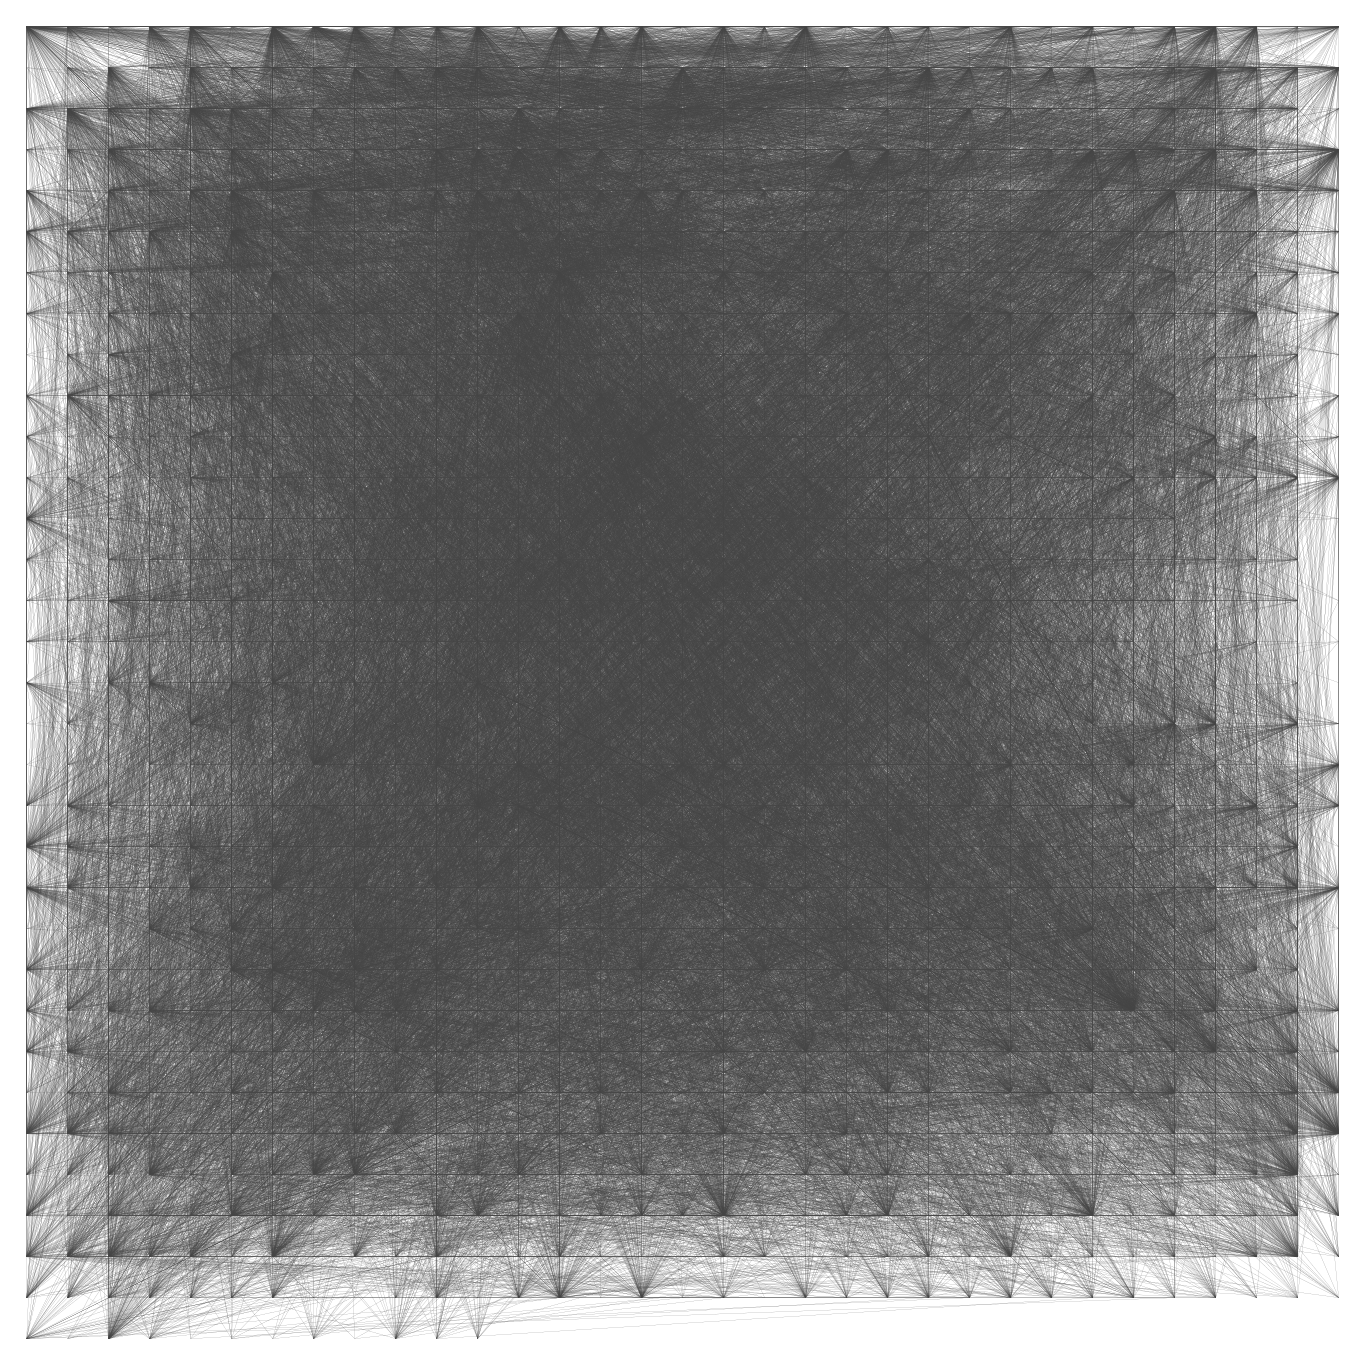
\includegraphics[width=\columnwidth]{src/youtube/hdg/comp/4_plot_frgrid}\\
  \captionof{figure}{Fruchterman Reingold grid layout}
  \label{fig:hdg_c4}}
\end{multicols}
\begin{multicols}{2}
  {\centering
  
\includegraphics[width=\columnwidth]{src/youtube/hdg/comp/5_plot_drl}\\
  \captionof{figure}{DrL layout}
  \label{fig:hdg_c5}}
  {\centering
  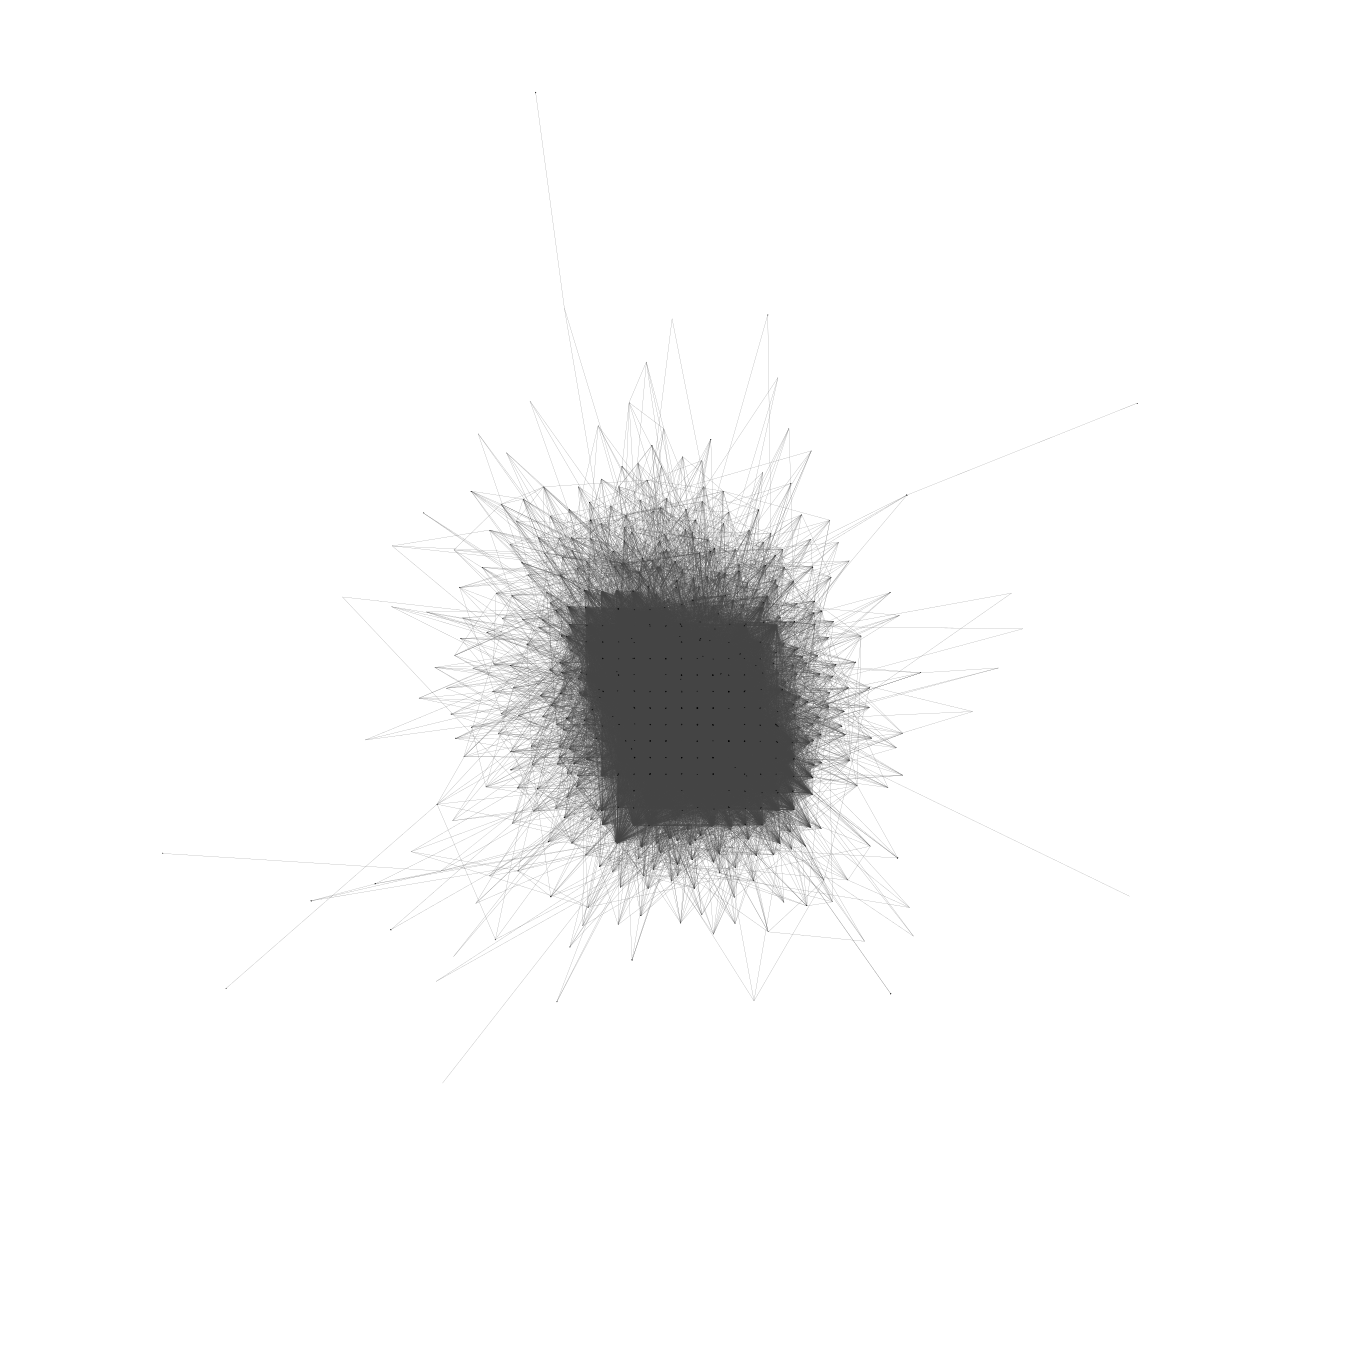
\includegraphics[width=\columnwidth]{src/youtube/hdg/comp/6_plot_ghopt}\\
  \captionof{figure}{Ghopt layout}
  \label{fig:hdg_c6}}
\end{multicols}
\begin{multicols}{2}
  {\centering
  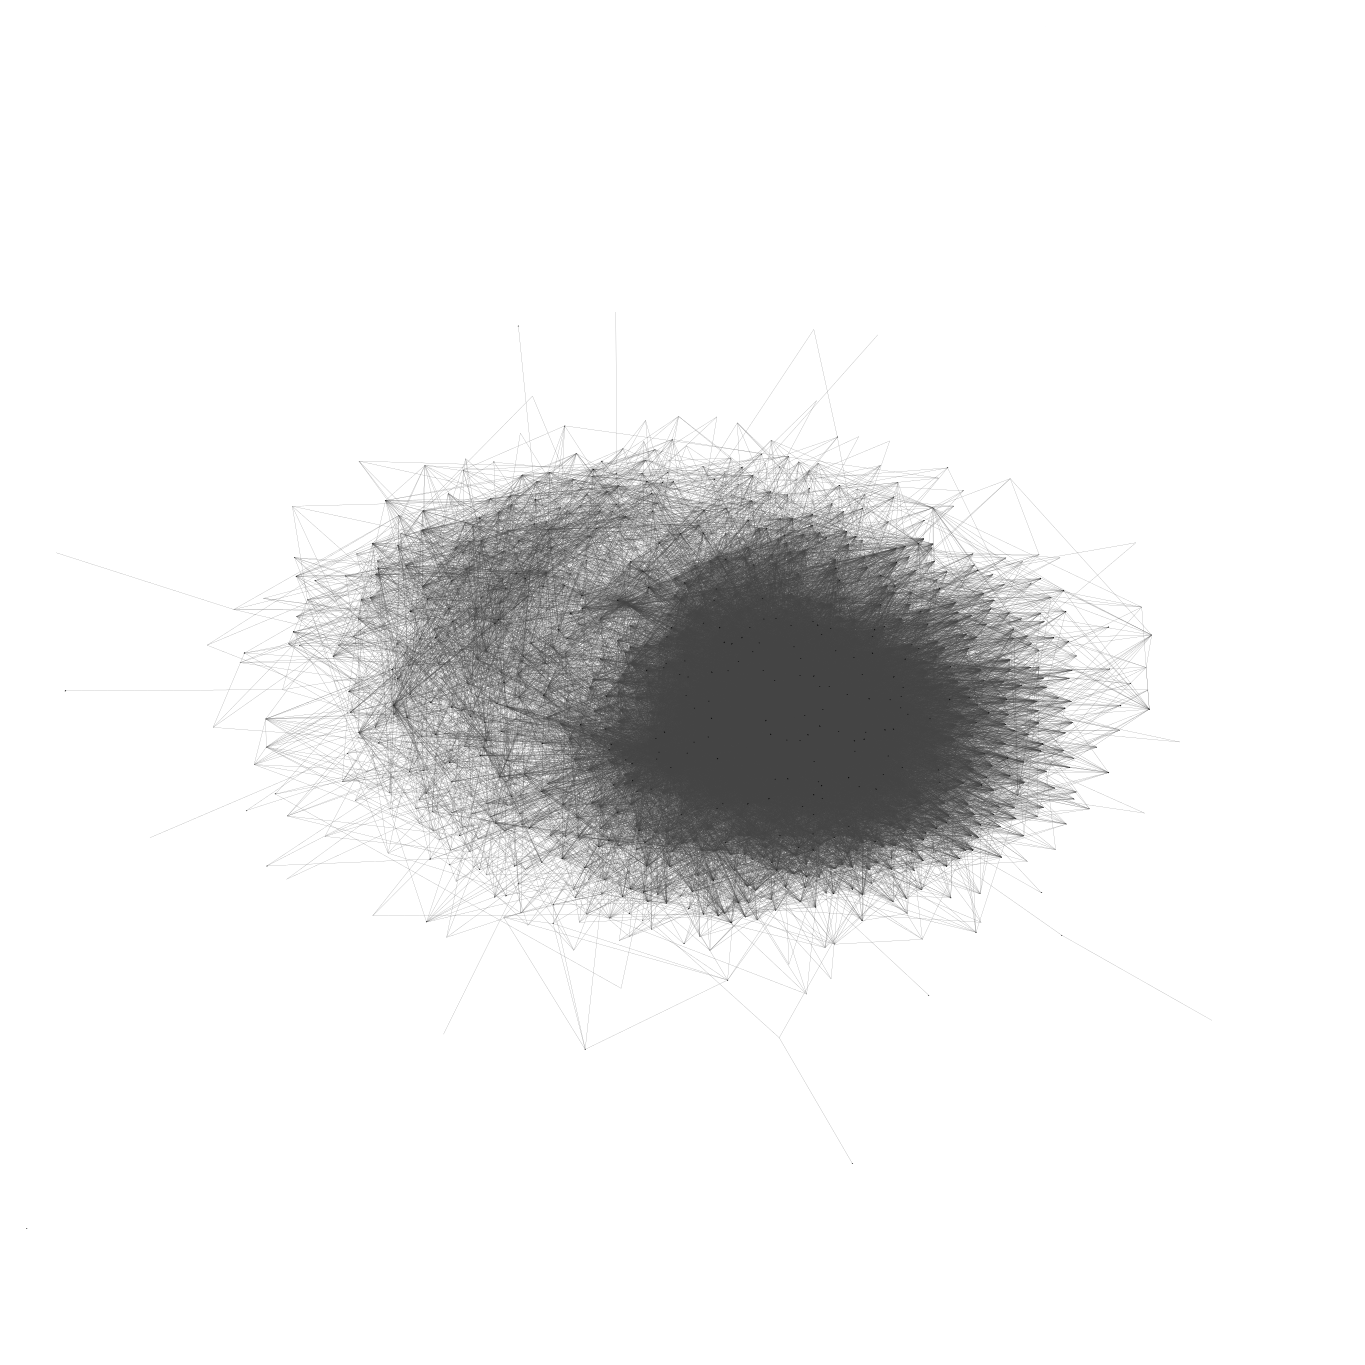
\includegraphics[width=\columnwidth]{src/youtube/hdg/comp/7_plot_kk}\\
  \captionof{figure}{Kamada Kawai layout}
  \label{fig:hdg_c7}}
  {\centering
  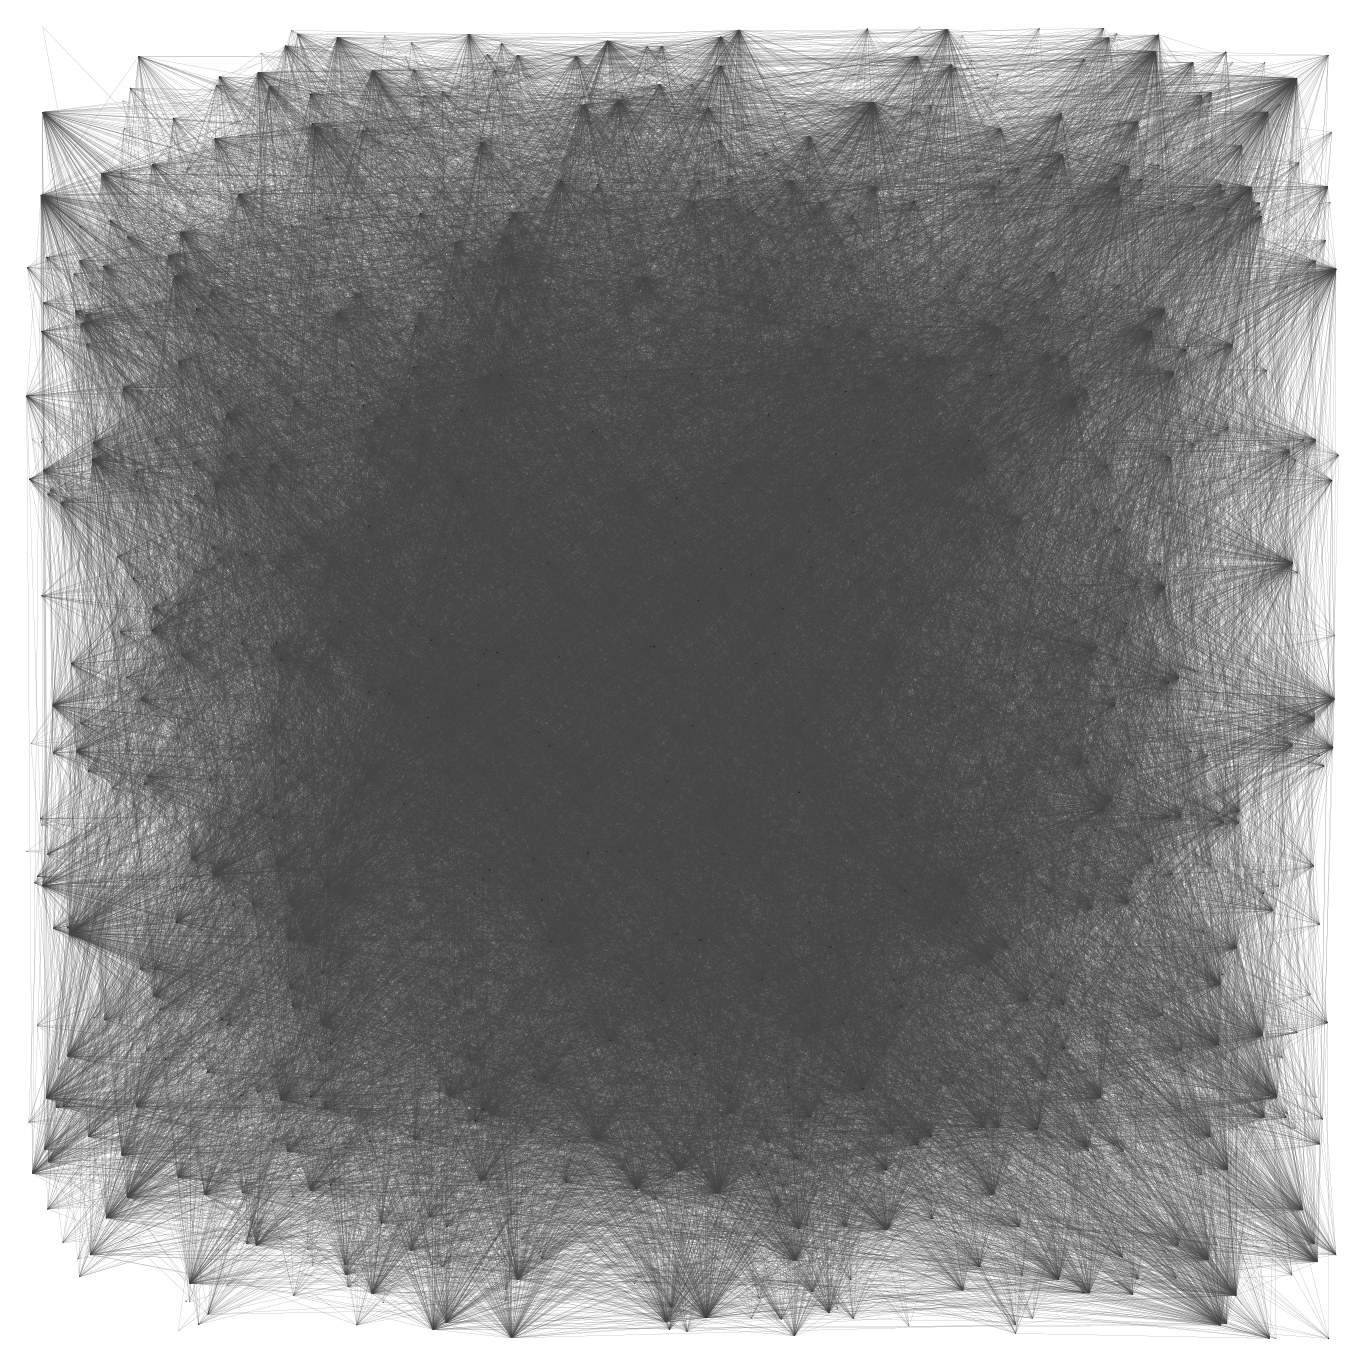
\includegraphics[width=\columnwidth]{src/youtube/hdg/comp/8_plot_random}\\
  \captionof{figure}{Random layout}
  \label{fig:hdg_c8}}
\end{multicols}
\begin{multicols}{2}
  {\centering
  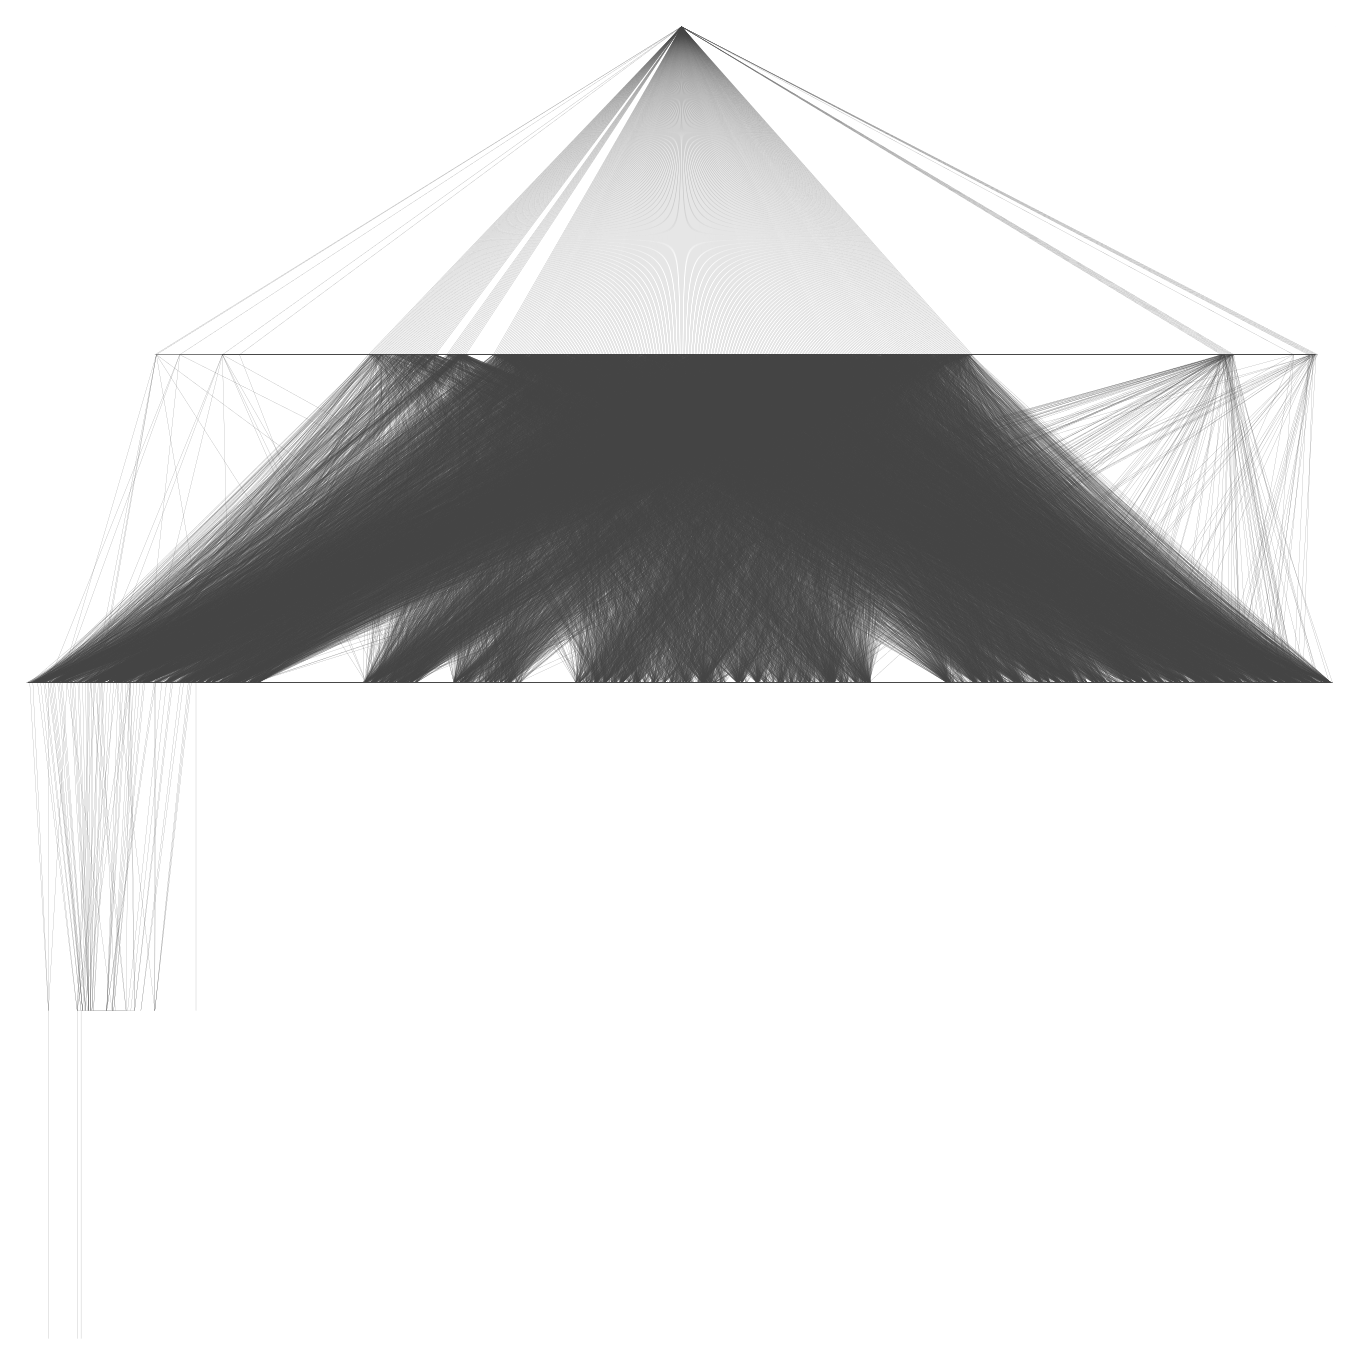
\includegraphics[width=\columnwidth]{src/youtube/hdg/comp/9_plot_sgy}\\
  \captionof{figure}{Sugiyama layout}
  \label{fig:hdg_c9}}
  \ \\
  \ \\
\end{multicols}

%- - - - - - - - - - - - - - - - - - - - - - - - - - - - - - - - - - - - - - - -
\subsubsection{Community plot}
%- - - - - - - - - - - - - - - - - - - - - - - - - - - - - - - - - - - - - - - -
\myparagraph{Clustering the subgraph}

The size of the subgraph we're clustering is smaller than the one used in the datashader example (only \improvement{list the number of nodes} nodes), so we can use the infomap clustering algorithm on it right away.

\listcode[src/youtube/hdg_com/1_clustering.py]{Using infomap to cluster the subgraph}

\myparagraph{Making communities visible}

There are a couple of ways to make communities in your graph more visible on the resulting plot. You could (1) use color to distinguish between them, (2) draw vertices from one community close to each other, (3) separate communities by drawing their boundaries, or (4) label each vertice with their community label. Some of those techniques are only effective when applied to very small graphs (like labeling), while other are a better fit for a medium-sized graph like the one used in this example.

\listcodecont[src/youtube/hdg_com/2_initializing_colors.py]{Initializing color and weight lists}

Something about the algorithm here.

\listcodecont[src/youtube/hdg_com/3_colors_looping_vert.py]{Assigning color to vertices}

\listcodecont[src/youtube/hdg_com/4_colors_looping_edge.py]{Assigning color to edges}

\myparagraph{Styling the resulting plot}

Something about using graph properties to style the plot.

\listcodecont[src/youtube/hdg_com/5_styling_prop.py]{Styling using graph properties}

Something about using the style dictionary to style the plot.

\listcodecont[src/youtube/hdg_com/6_style_dict.py]{Styling using a style dict}

\myparagraph{Plotting and reviewing the results}

Something about the plot.

\listcodecont[src/youtube/hdg_com/7_plotting.py]{Saving the plot to a file}

\begin{figure}[p]
    \centering
    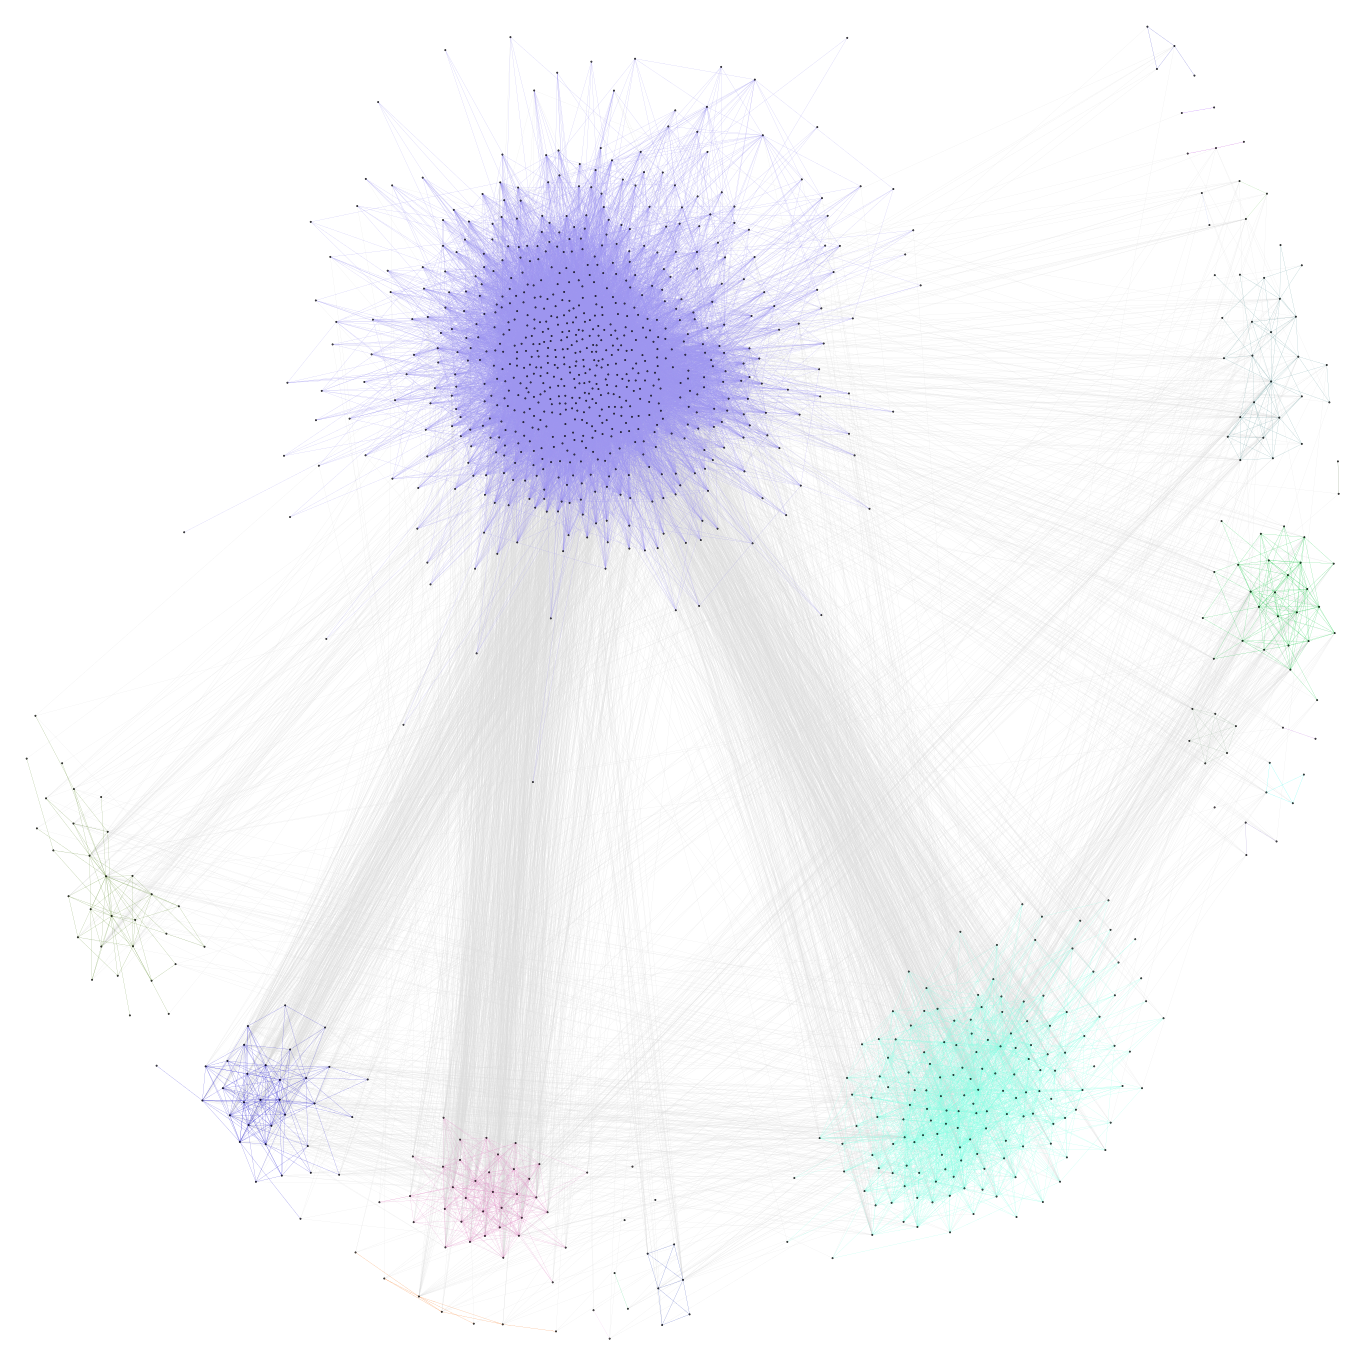
\includegraphics[width=\textwidth]{src/youtube/hdg_com/hdg_com}
    \caption{Community plot}
    \label{fig:hdg_com}
\end{figure}

\begin{figure}[p]
    \centering
    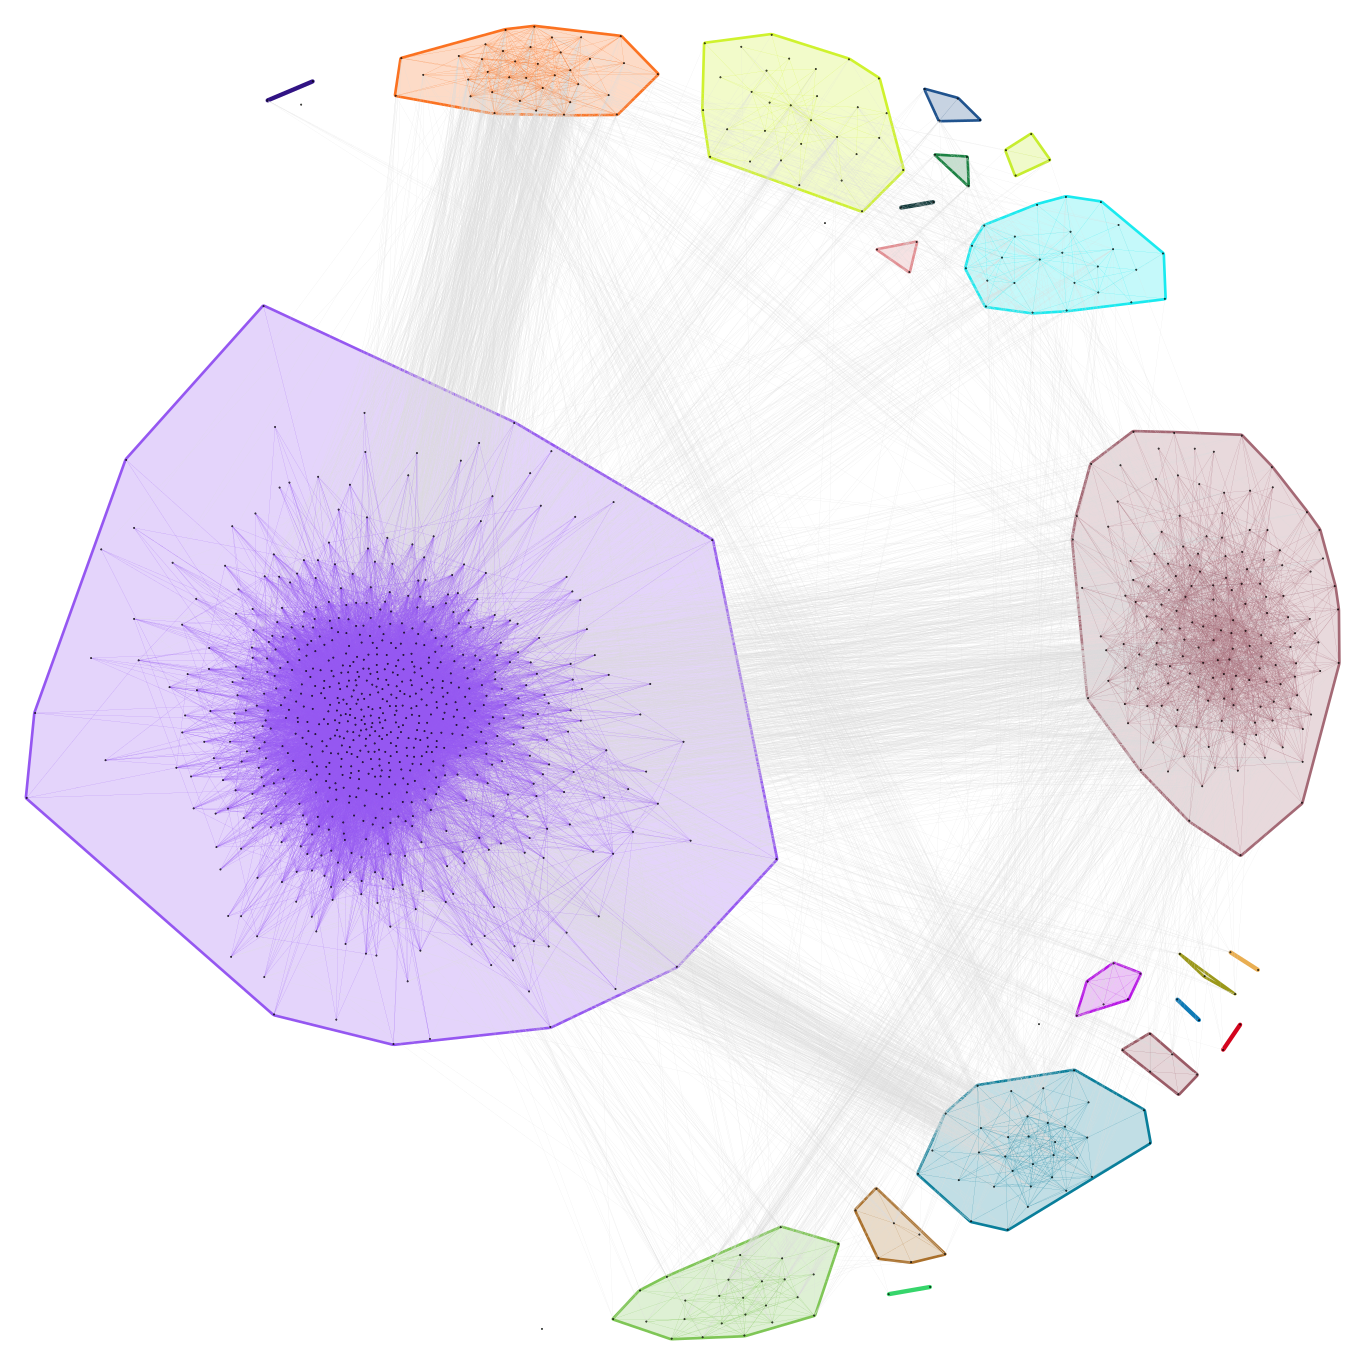
\includegraphics[width=\textwidth]{src/youtube/hdg_com/hdg_com_marked}
    \caption{Community plot - marked groups}
    \label{fig:hdg_com_marked}
\end{figure}

%- - - - - - - - - - - - - - - - - - - - - - - - - - - - - - - - - - - - - - - -
\subsubsection{Weighted community plot}
%- - - - - - - - - - - - - - - - - - - - - - - - - - - - - - - - - - - - - - - -
\myparagraph{Pagerank application}

Pagerank \improvement{cite} is an algorithm developed by google.

\listcode[src/youtube/hdg_weighted/1_pagerank.py]{Using pagerank to assign weights to vertices}

%
\myparagraph{Style dictionary}

Style dictionary for the weighted graph is very similar to the one that was used to create the regular community plot, with an addition of ...

\listcodecont[src/youtube/hdg_weighted/2_style_dict.py]{Styling using a style dict}

%
\myparagraph{Plotting and reviewing results}

\listcodecont[src/youtube/hdg_weighted/3_plotting.py]{Saving the plot to a file}

\begin{figure}
    \centering
    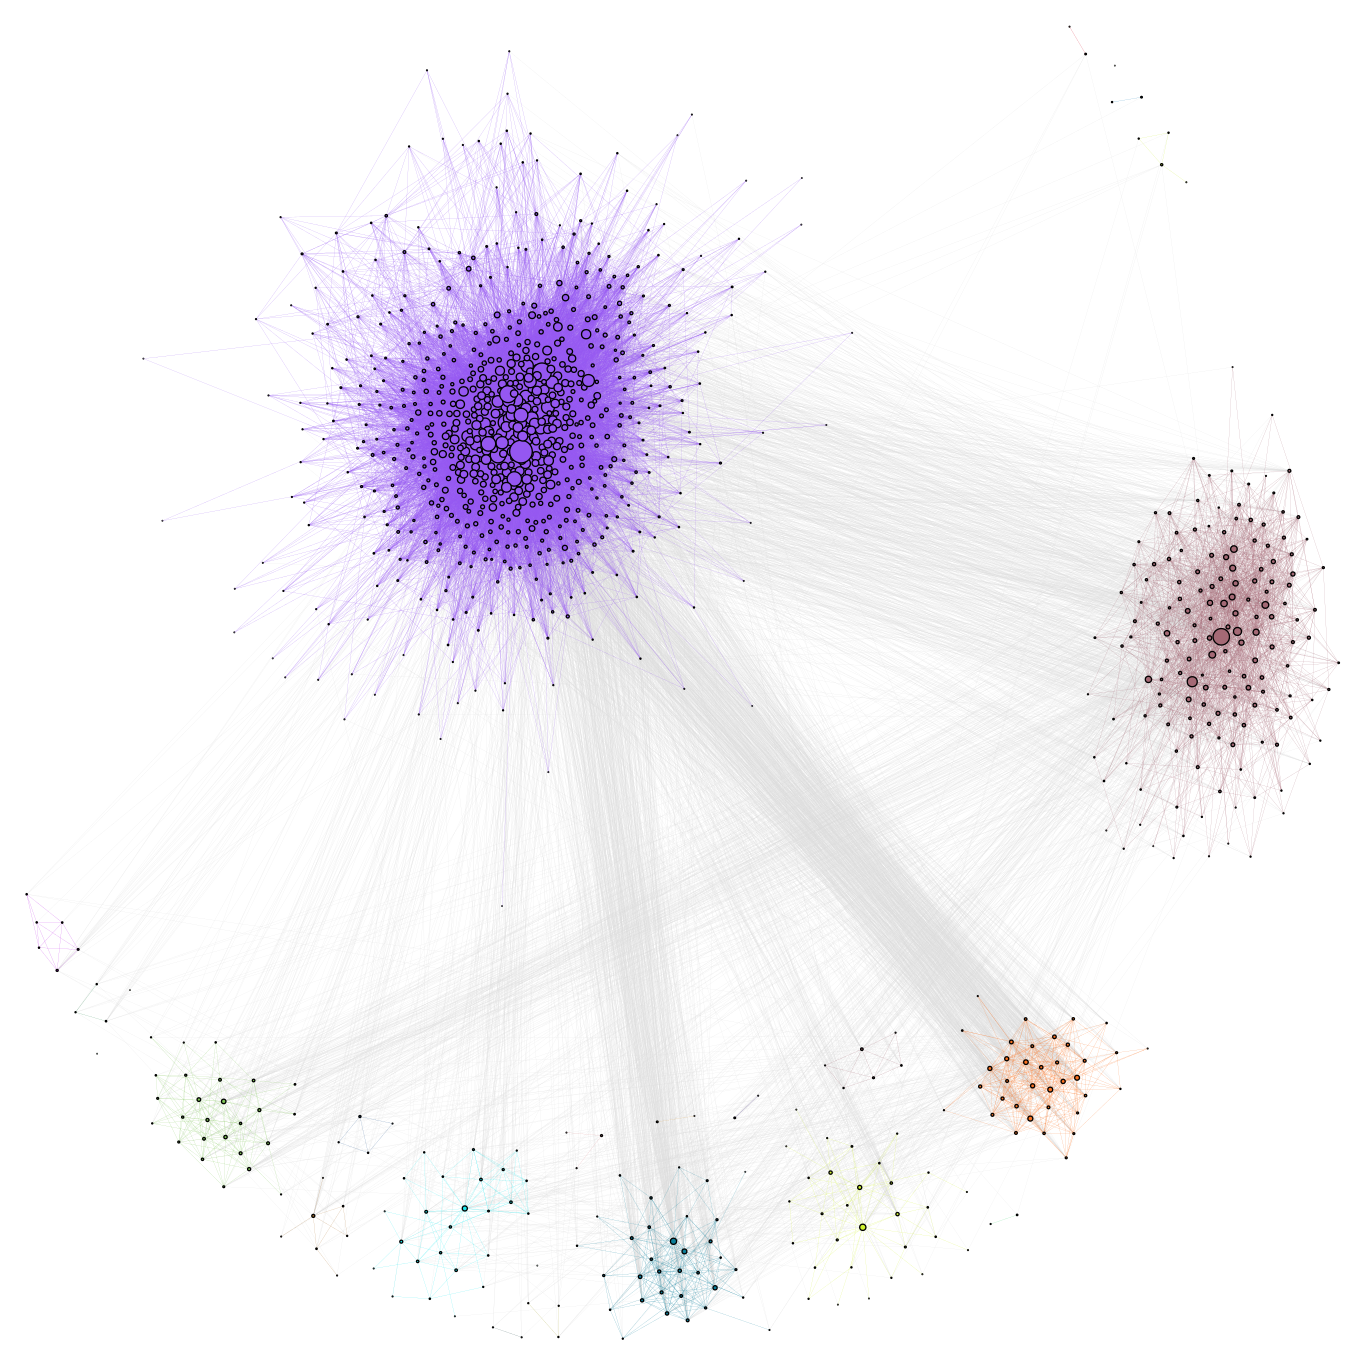
\includegraphics[width=\textwidth]{src/youtube/hdg_weighted/hdg_pg_fg}
    \caption{Weighted plot - Fruchterman Reingold layout}
    \label{fig:hdg_pg_fg}
\end{figure}

\begin{figure}
    \centering
    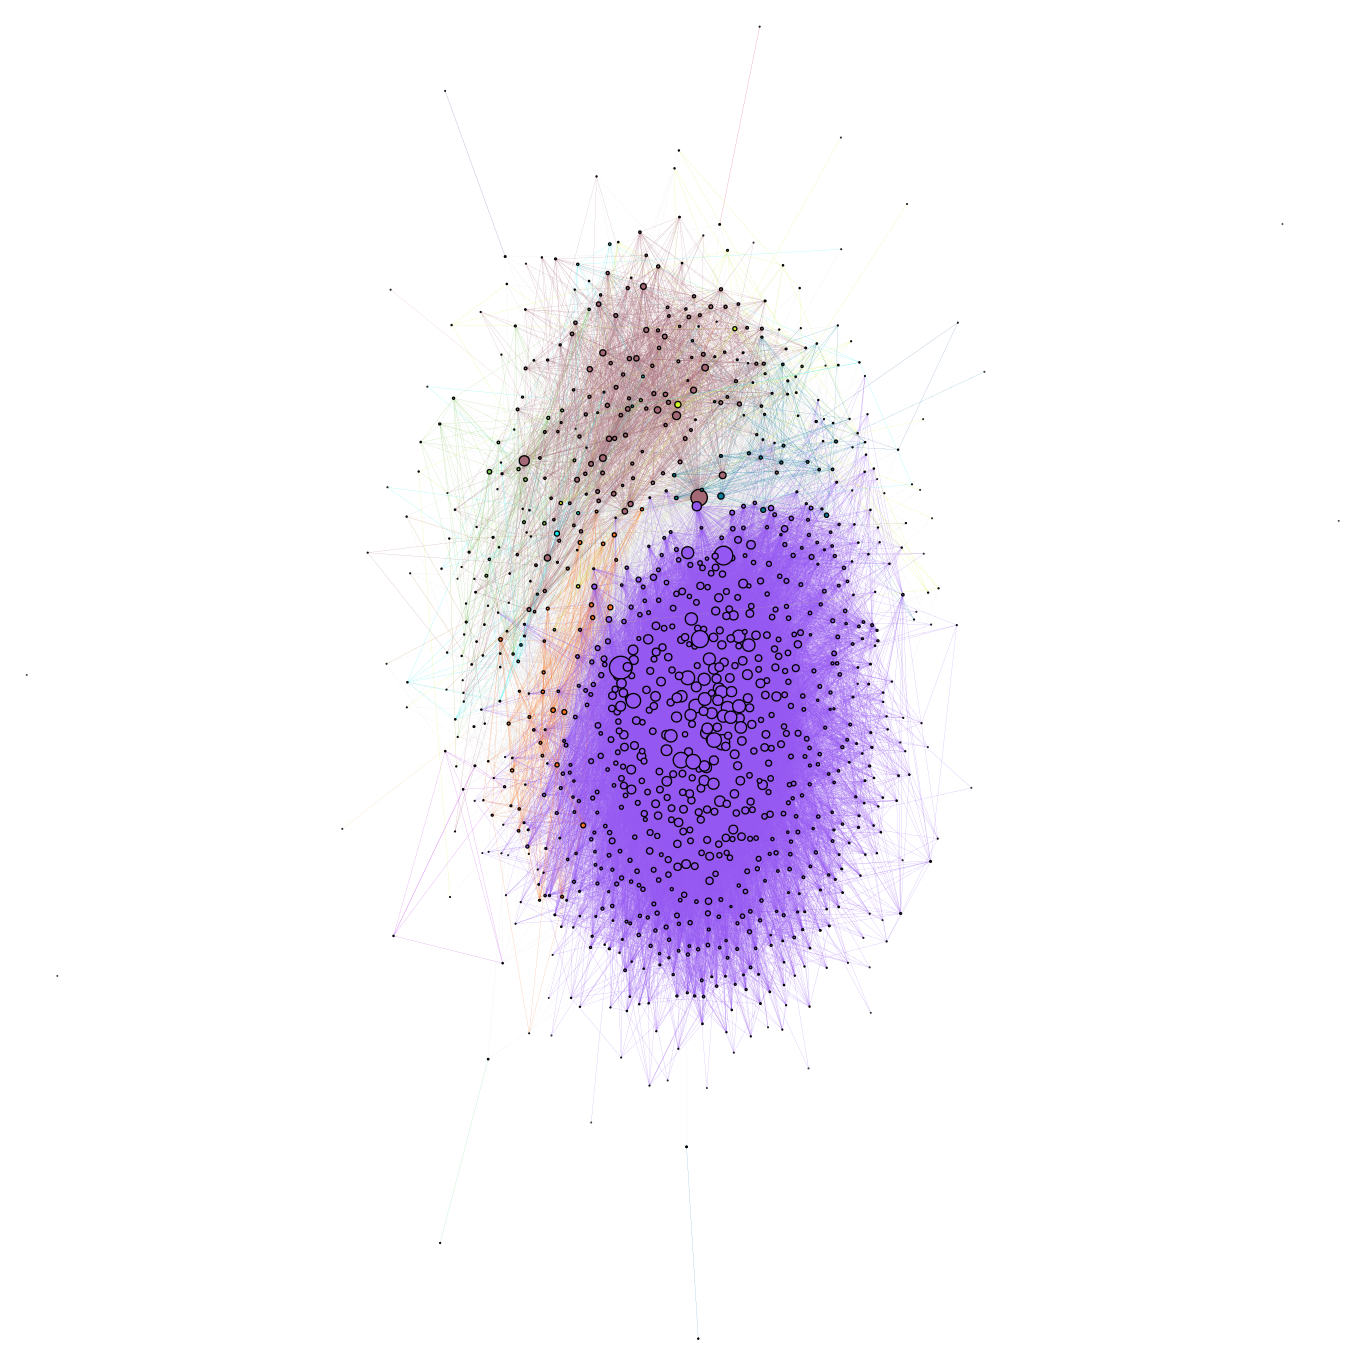
\includegraphics[width=\textwidth]{src/youtube/hdg_weighted/hdg_pg_kawai}
    \caption{Weighted plot - Kamada Kawai layout}
    \label{fig:hdg_pg_kawai}
\end{figure}



%===============================================================================
\newpage
\section{GEODATA ANALYSIS}
%===============================================================================

%-------------------------------------------------------------------------------
\subsection{Project Overview}
%-------------------------------------------------------------------------------
\begin{easylist}
# Goals
## to show how to deal with geodata in python
# Plots
## KPI per country (Basemap)
## Plot - KPI per state in a country (libnamehere)
## Plot - Chikago Taxi (datashader)
\end{easylist}






% Literature references
\newpage
\nocite{*}
\bibliographystyle{unsrt}
\bibliography{references}

\end{document}
